% UG project example file, February 2022
% Do not change the first two lines of code, except you may delete "logo," if causing problems.
% Understand any problems and seek approval before assuming it's ok to remove ugcheck.
\documentclass[logo,bsc,singlespacing,parskip]{infthesis}
\usepackage{ugcheck}
\newcommand{\todo}{\textbf{?} }
\usepackage{color,soul}
% \usepackage{hyperref}
\usepackage{graphicx}
\usepackage{array}
\usepackage{xcolor}
\usepackage{soul}
\usepackage{booktabs}
\usepackage{fancyvrb}
\usepackage{relsize}
\usepackage{float}

\newenvironment{VerbatimCompact}
  {\vspace*{-2.5mm}\VerbatimEnvironment
   \par\Verbatim}
  {\endVerbatim\vspace*{-2.4mm}}


\newcolumntype{V}[1]{>{\topsep=0pt\@minipagetrue}p{#1}<{\vspace{-\baselineskip}}}
\makeatother
\newcommand{\command}[1]{\texttt{\string#1}}

\newcommand{\hlc}[2][yellow]{{%
    \colorlet{foo}{#1}%
    \sethlcolor{foo}\hl{#2}}%
}

\newcolumntype{L}[1]{>{\raggedright\let\newline\\\arraybackslash\hspace{0pt}}m{#1}}
\newcolumntype{C}[1]{>{\centering\let\newline\\\arraybackslash\hspace{0pt}}m{#1}}
\newcolumntype{R}[1]{>{\raggedleft\let\newline\\\arraybackslash\hspace{0pt}}m{#1}}

\newenvironment{compactlist}
{ \begin{enumerate}
    \setlength{\itemsep}{0pt}
    \setlength{\parskip}{0pt}
    \setlength{\parsep}{0pt}     
}
{ \end{enumerate} } 

% Include any packages you need below, but don't include any that change the page
% layout or style of the dissertation. By including the ugcheck package above,
% you should catch most accidental changes of page layout though.

\usepackage{microtype} % recommended, but you can remove if it causes problems

\begin{document}
\begin{preliminary}

\title{Efficient MLIR Compiler Design: Vectorization for Presburger Library}

\author{Zhou Qi}

% CHOOSE YOUR DEGREE a):
% please leave just one of the following un-commented
% \course{Artificial Intelligence}
%\course{Artificial Intelligence and Computer Science}
%\course{Artificial Intelligence and Mathematics}
%\course{Artificial Intelligence and Software Engineering}
%\course{Cognitive Science}
\course{Computer Science}
%\course{Computer Science and Management Science}
%\course{Computer Science and Mathematics}
%\course{Computer Science and Physics}
%\course{Software Engineering}
%\course{Master of Informatics} % MInf students

% CHOOSE YOUR DEGREE b):
% please leave just one of the following un-commented
%\project{MInf Project (Part 1) Report}  % 4th year MInf students
%\project{MInf Project (Part 2) Report}  % 5th year MInf students
\project{4th Year Project Report}        % all other UG4 students


\date{\today}

\abstract{
\label{sec:abstract}

This report presents a faster implementation for the core \texttt{pivot}
function of MLIR’s presburger library. Its hot loop is element-wise
overflow-checked multiplication and addition on an input matrix of low dimension
and mostly small value elements. 

The current approach of upstream is element-wise multiplication and addition  on
transprecision integer matrices, from \texttt{int64\_t} to
\texttt{LargeInteger}. This can be improved by efficiently utilizing hardware
resources, taking advantage of SIMD, and reducing the bit width for every
element: the compiler is not capable of automatically generating vectorized
instructions for element-wise transprecision computing, and \texttt{int64\_t}
has a much larger bit width than what is typically used for most of the elements
in the matrix. Additionally, extra arithmetics are required to perform overflow
checking for \texttt{int64\_t}, resulting in significant performance overhead.
This report “innovates” the \texttt{int23\_t} \footnote{This is not really a
innovation. It it a common technique on GPUs because often they are more capable
on floating points than integers. See Section \ref{sec:introduction} for more
history and detail. } datatype, a 23-bit integer datatype that utilizes the
23-bit mantissa of a 32-bit floating point, to address these issues. The faster
“pivot” performs matrix-wise transprecision computing, targeting 99\% \hl{TODO:
confirm this number} of the case where elements fit inside \texttt{int23\_t}.
Overflow awareness overhead is almost free, as floating point imprecision
implies \texttt{int23\_t} overflow (See Section \ref{sec:todo}) and can be
captured by a status register. It takes as low as 1 ns to check the status
register in the pipeline, and only takes 9 ns to reset the status register.
Additionally the status register is only cleared once before a sequence of
\texttt{pivot} calls, making the average cost of clearing the status register
per \texttt{pivot} negligible.  
    
On a 30-row by 16-column example matrix, it performs 30 times faster than the
upstream scalar implementation. The time cost of a single \texttt{pivot} call is
reduced from 550 ns to 18.6 ns. \hl{TODO: replace this with actual MLIR benchmark
result}

\hl{TODO:Question: mention int16 here?}

\hl{TODO:Reminder: we don't use int16 for (1) compatibility (2) only slightly faster than float}

}

\maketitle

\newenvironment{ethics}
   {\begin{frontenv}{Research Ethics Approval}{\LARGE}}
   {\end{frontenv}\newpage}

\begin{ethics}

This project was planned in accordance with the Informatics Research
Ethics policy. It did not involve any aspects that required approval
from the Informatics Research Ethics committee.

\standarddeclaration
\end{ethics}


\begin{acknowledgements}
    First and foremost, I would like to express my deepest gratitude to my
    supervisor, Tobias Grosser, for his unwavering support, guidance, and
    encouragement throughout the course of this research. His extensive
    knowledge, valuable insights, and patience have been instrumental in shaping
    my academic and personal growth.

    I am also immensely grateful to Arjun Pitchanathan, a fellow Ph.D. student
    under the supervision of Tobias Grosser, for his invaluable assistance and
    collaboration. His expertise, constructive feedback, and willingness to
    share his knowledge have significantly contributed to the progress and
    quality of this work.
    
    Furthermore, I would like to acknowledge the generous contributions from
    Marisa Kirisame, Emanon, gjz010, and lyzh, whose insightful comments,
    technical support, and camaraderie have enriched my research experience.
    Their shared wisdom and passion for the subject matter have made this
    journey both enjoyable and rewarding.
    
    Finally, I am thankful to all my friends, colleagues, and family members who
    have provided me with the emotional support and encouragement needed to
    complete this paper. Their unwavering belief in my abilities has been a
    source of strength and motivation throughout this challenging process.
\hl{TODO:}

\end{acknowledgements}


\tableofcontents
\end{preliminary}


\chapter{Introduction}
\label{sec:introduction}

MLIR, Multi-Level Intermediate Representation, is a infrastructure for building
reusable and extensible compilers. Its aim is to reduce fragmentation in domain
specific languages and heterogeneous hardwares \cite{mlir}. Its Presburger
library provides polyhedral compilation techniques to make dependence analysis
and loop optimization \cite{mliraffine} and cache modeling \cite{CacheModel}.
Presburger arithmetics involves determining whether conjunction of linear
arithmetic constraints is satisfiable \cite{SMLPPA}, and can be solved using the
simplex method of linear programming, with its core function "pivot" consumes
\hl{TODO: find the number} \% \cite{FPL1} of the runtime. 

The \texttt{pivot} function involves two multiplication and one addition
operation on every element in a matrix. Notably, the input matrices for this
library tend to exhibit characteristics of small values and low dimensionality.
For example, 90\% of test cases work with 16-bit integers that never overflow,
and 74\% of isl’s runtime is spent on test cases that we can compute using
16-bit integers and matrices with at most 32 columns \cite{FPL2}. These
properties can be leveraged to take advantage from modern micro-architectural
hardware resources, thereby accelerating the process.

Currently, the source code in MLIR upstream adopts a nested for-loop to iterate
through every element of the matrix in a transprecision manner. Each number in
the matrix can either be \texttt{int64\_t} or \texttt{LargeInteger}. The
algorithm starts by using \texttt{int64\_t}, in case of overflow, it switches to
the \texttt{LargeInteger} version. This approach is computationally expensive
and inefficient, for the following reasons: 
\begin{enumerate}

\item \texttt{int64\_t} has a much larger bit width than what is typically
used for most of the elements in the matrix,

\item the compiler is not capable of automatically generating vectorized
instructions to further optimize the process,

\item overflow is checked manually through additional arithmetic
operations.

\end{enumerate}

To propose a faster alternative of the \texttt{pivot} function, we could
consider constructing a new \texttt{pivot} algorithm that satisfies the
following conditions:
\begin{enumerate}

\item Utilize SIMD: preliminary benchmarks (see Section \ref{sec:todo}) indicate
8x \hl{TODO: verify this number} performance improvement on a simple vector
element-wise add example. 

\item Use small bit width for every element: reducing bit width by half doubles the
amount of numbers packed into a single vector register, and essentially reduces
the instruction count by half.  \hl{(Some figure TODO)}

\item Fast overflow checking: for integers, overflow has to be checked manually
and this introduces 60\%  \hl{(TODO: verify this number?)} overhead, as
benchmarks in the Section \ref{sec:todo} shown. This is because the x86
architecture does not provide status registers to indicate integer overflown.
However, there is one for floating points, making floating points overflow
detection almost free. 

\end{enumerate}


opencompl’s fork of LLVM includes a modified version of \texttt{pivot} that
utilizes \texttt{int16\_t} and is designed for matrices with 32 columns or less \cite{FPL2}.
This approach offers the advantage of being able to pack a row of 32 elements
into a single \texttt{AVX-512} register and addresses issues 1 and 2. However,
overflow is still checked manually, causing 4x or 5x more instruction count (
Section \ref{sec:todo}). Moreover, this approach introduces a new disadvantage,
the support for vectorized \texttt{int16\_t} is very rare among CPU manufactured
in the last decade (Section \ref{sec:todo}). 

An alternative approach is to do 23-bit or 52-bit integer operations using float
(32-bit floating point) or double (64-bit floating point) respectively. Though
floating points are notorious for precision issues, they are reliable when
representing integers that fit inside their mantissa, 23 bits for float and 52
bits for double \footnote{ IEEE 754 specification is introduced in Section
\ref{sec:todo}}. When the result of some integer computation exceeds the bit
size of the mantissa, floating point imprecision almost always occurs and a
status register will be set automatically (Section \ref{sec:todo}). Comparing to
\texttt{int16\_t}, even though vector size is sacrificed as there does not exist
support for 16-bit floating point \texttt{half}, using floating points could
still potentially be faster, because overflow checking overhead can be
significantly reduced. With floating points, the cost of overflow checking is
the time spent on resetting the status register once at the beginning of a
sequence calls to `pivot`, plus reading it, per \texttt{pivot} call. Benchmarks
\hl{TODO: some figure} indicate that the total overhead is as low as 1 ns, as it
only adds 1 ns to read the status register in the instruction execution
pipeline, and the average cost of resetting per pivot is negligible. 

This report will first analyze the capability of modern CPU micro-architecture,
especially \texttt{Zen4}, through a matrix element-wise fused-multiply-add toy
example under the various configurations regarding vectorization methods, matrix
data structures, element data types and data widths (Section \ref{sec:Toy}). 

It is discovered that optimal performance can be achieved by selecting clang
builtin vector type as vectorization methods and use flat list as matrix data
structure. However, it is quite difficult to decide whether \texttt{int16\_t} or
\texttt{float} is better, because the former benefits form bigger vector size
and less instruction count, while the latter has minimal overhead on overflow
checking. 

Then two detached versions of \texttt{pivot} function from the Presburger
library are built from the most optimal configurations derived form the toy
example, one using \texttt{int16\_t} and the other using \texttt{float}. Some
further optimizations were made by inspecting \texttt{perf} reports and
assembly, including: 

\begin{compactlist} 
    \item Reduce memory operation
    \item Unroll loops
    \item\hl{TODO: what are the other optimizations?}
\end{compactlist}

\hl{TODO: Update here after Integrating into library}



\chapter{Background}
\section{Presburger library}
% \subsection{Overview}

The FPL paper obtained 465,460 representative linear problems encountered during
integer set coalescing by analyzing linear programs in cache analytical
modeling, polyhedral loop optimization, and accelerator code generation. It is
found that most of the constraint matrices are low in dimensionality and small
in the value of each element. Specifically, more than 99\% of the coefficients
require less than 10 bits and 95\% of them are less than 20 columns \cite{FPL1}.
Thus, most of the rows fit inside a 512-bit vector register of 32
\texttt{int16\_t} elements, and a row operation can be done in a single
instruction. 

However, in rare and corner cases, there can be larger coefficients up to 127
bits. Practically, the upper bound of coefficient size is unknown, making it
required to have arbitrary precision arithmetic \texttt{LargeInteger} as a
backup. Also, the maximum observed column count is 28 and there is not a certain
maximum column count as well. 

Therefore the FPL paper presents a 3-way transprecision implementation for the
Presburger library, from row-wise vectorized \texttt{int16\_t} to element-wise
scalar \texttt{int64\_t} and element-wise scalar \texttt{LargeInteger}, as
illustrated in Figure \ref{fig:fpl_arch}. But unfortunately the MLIR upstream
only presents a 2-layer transprecision, consisting of element-wise scalar
operation using \texttt{int64\_t} and \texttt{LargeInteger}. The
\texttt{int16\_t} version is not merged with the upstream for two reasons: 
\begin{compactlist} 
    \item \texttt{int16\_t} vectors require AVX-512 ISA extension, but hardware
    support are rare (Section \ref{sec:avx512}). 
    \item Despite the \texttt{int16\_t} version is fast \hl{TODO: find how much
    faster in FPL paper}, overflow checking overhead is ??\%\hl{TODO: find how
    much is overhead} \cite{FPL2}. Using floating points could significantly
    reduce this overhead and potentially be faster (Section \ref{sec:i23}).  
\end{compactlist}


\begin{figure}
    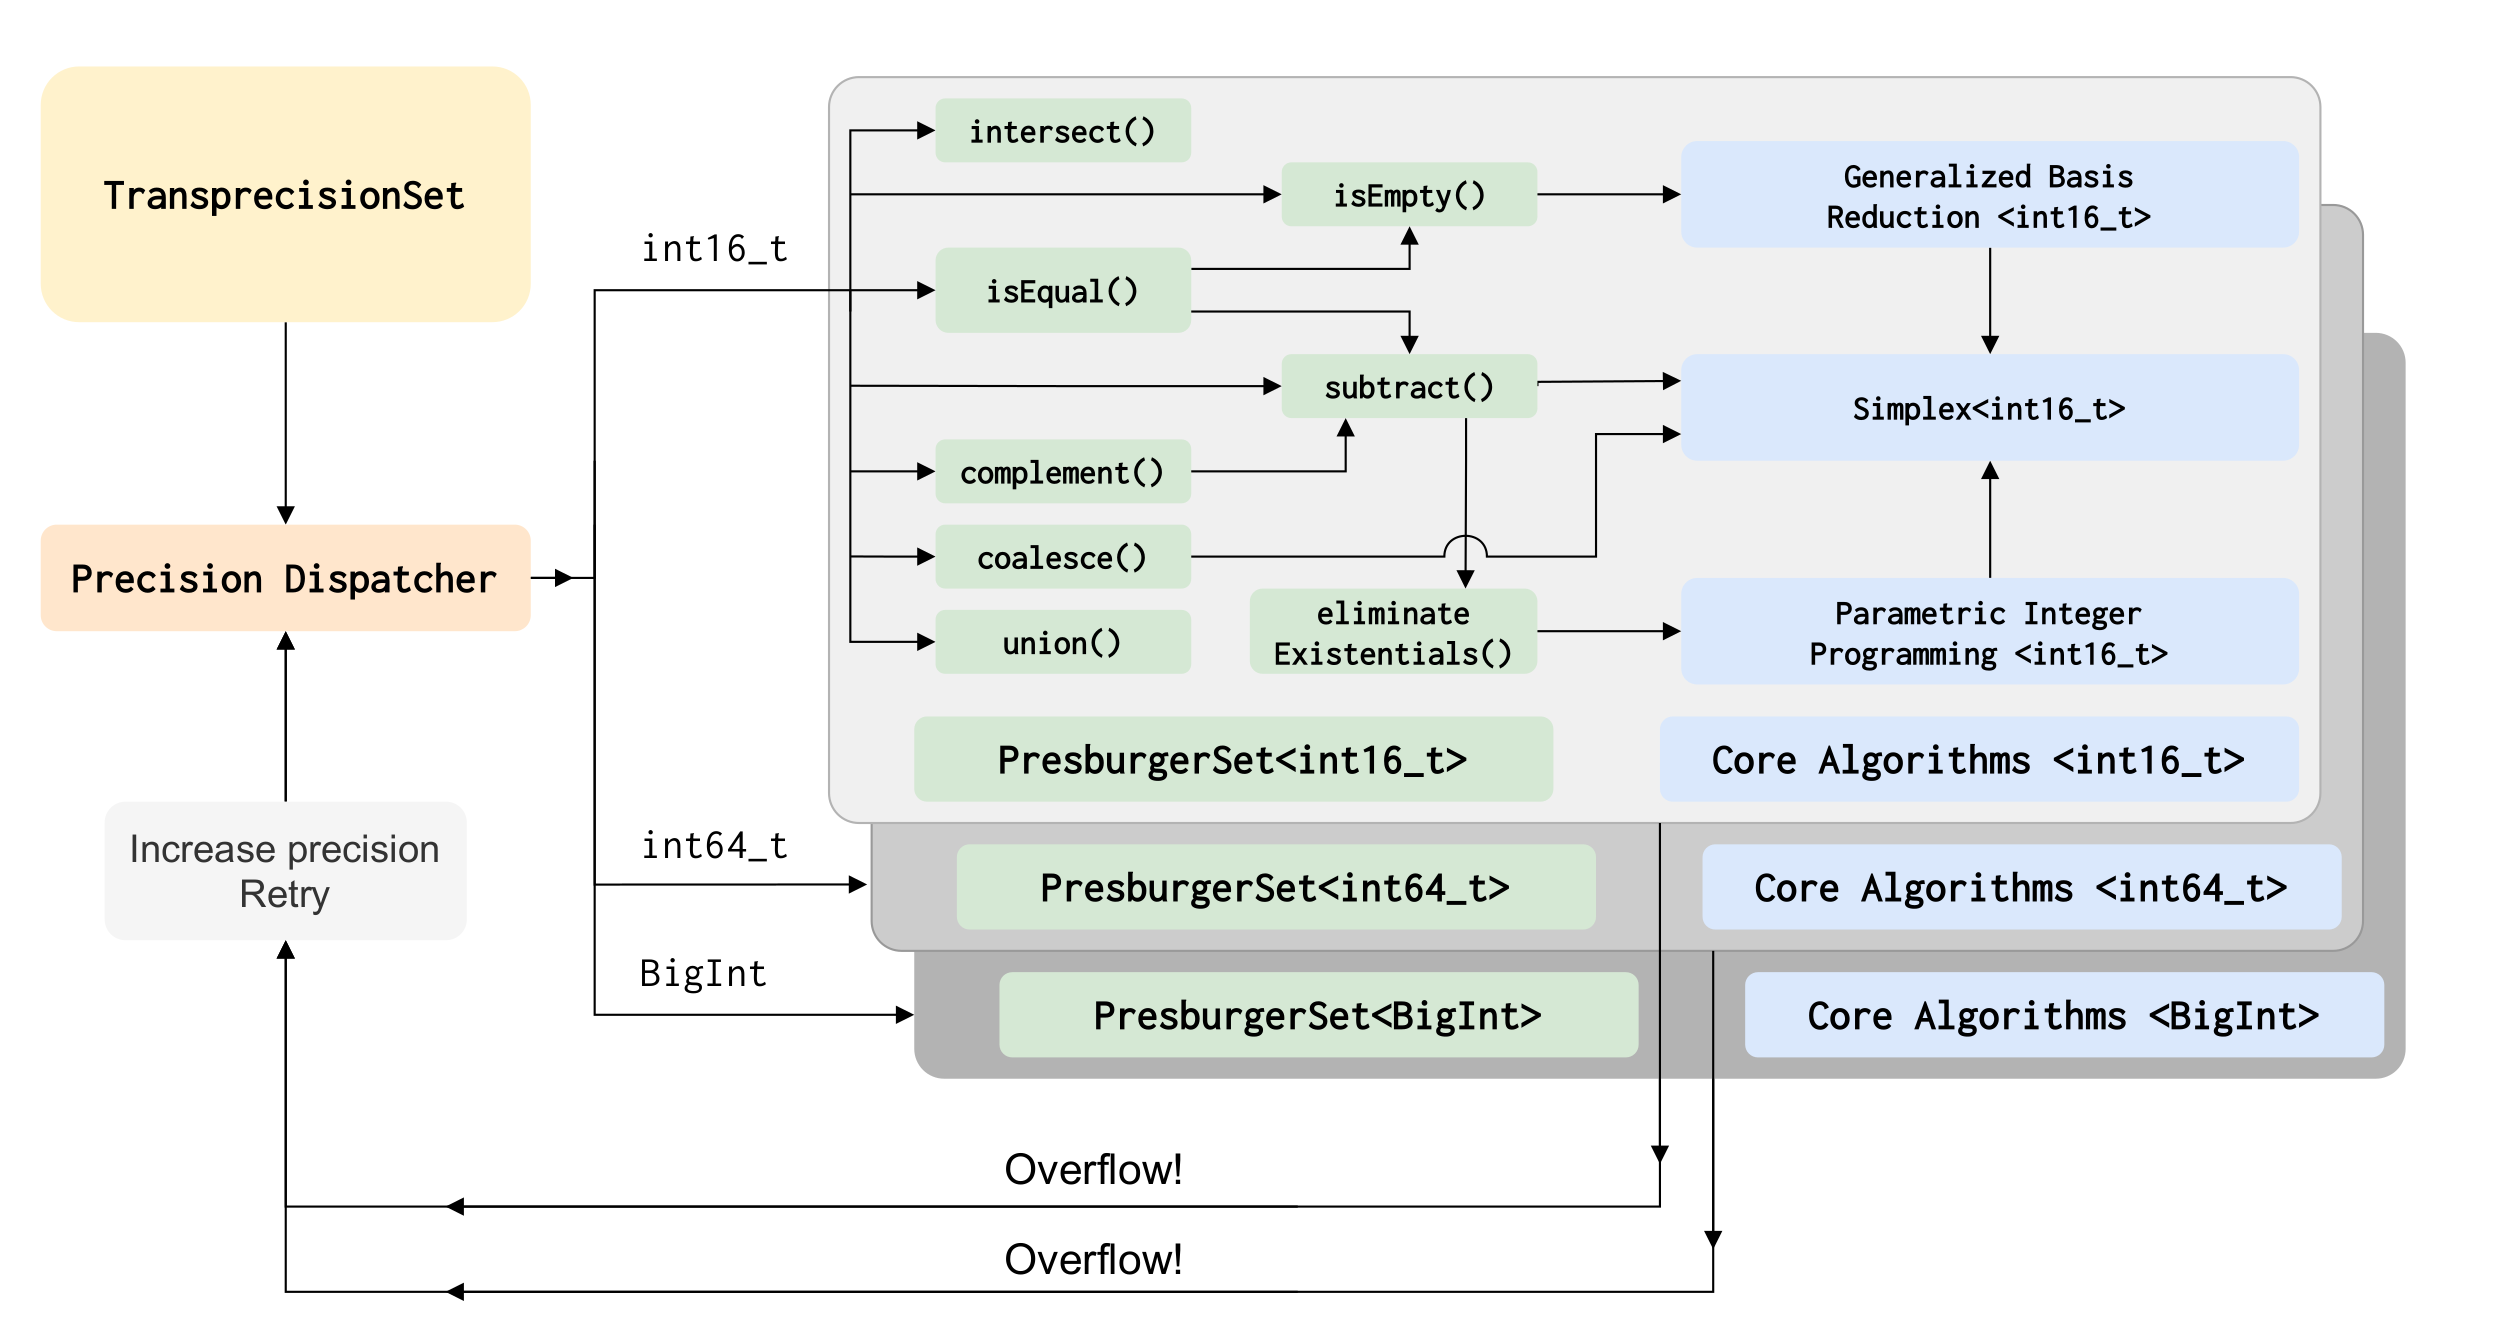
\includegraphics[width=\linewidth]{image/transprecision.png}
    \caption{The The architecture of FPL.}
    \label{fig:fpl_arch}
\end{figure}

\section{Modern CPU micro-architecture}
\label{sec:avx512}

A recent trend in x86-64 architecture’s development is to include AVX-512
instruction set architecture (ISA) extension. AVX-512 succeeds AVX2, the vector
width is increased from AVX-2’s 256 bits to 512 bits. AVX-512 also provides new
instructions, for example, \texttt{int16\_t} saturated addition.

% \subsection{History}

Even though its specification was released by Intel in 2013, it had been
unpopular, as it did not bring practical performance improvements. The primary
reason was that it consumed a lot more power than usual, causing severe
overheating. The micro-architecture Skylake from Intel, and its AVX-512 enabled
counterpart Skylake-X is a classic example. Skylake provides 2 256 bits FMA
AVX-2 execution units 
\footnote{Fused-multiply-add (FMA) execution units are a type of
floating point execution units, capable of doing addition, multiplication or
both in a single instruction. See Section \ref{sec:FMA}.} 
and Intel provides 2 512-bit AVX-512 FMA units by
fusing the existing AVX-2 units into a AVX-512 unit, then introduces an
additional FMA AVX-512 unit \cite{SLK-X}. The additional AVX-512 unit increases
the heat flux density of the chip, causing server thermal throttling issues. 

Intel attempted to mitigate this problem by introducing the ``AVX-offset'' mode.
When a workload involving AVX-512 instructions is encountered, the CPU
automatically enters AVX-offset mode and reduces its clock frequency
\cite{AVX-offset}. However, in practice it is more common to have a mix of
control flow, SSE and AVX-512 instructions, causing many scenario could run
faster if the additional AVX-512 is disabled (and does not thermal throttle)
\cite{Zen4Critique}.

AMD’s implementation of AVX-512 in Zen4 has slightly less computing power, but
much more efficient. Zen4 can be considered as modernized version of Zen3 or
Zen2, where Zen2 and Zen3 supports AVX2 by providing 2 FADD units
\footnote{Floating-point add units (FADD) can execute addition instructions
only. They may be considered as simplified FMA} and 2 FMA units of 256-bit width
\cite{Zen2ChipWiki}. Zen4 "double-pumps" these existing circuits to create a
single 512-bit FADD and a single 512-bit FMA, without introducing any new
execution units for floating point arithmetic \cite{Zen4Critique}. Zen2 and Zen3
are reputable for its high performance per watt \cite{ZenPerfPerWatt}, and it is
expected to be better on zen4 with more advanced lithography. Benchmarks
(\hl{TODO Some section}) indicate that this design indeed does not cause
throttling in AVX-512 workloads \cite{Zen4Critique}.

Additionally, rebuilding existing software to target AVX-512 may bring slight
performance improvement. One benefit of AVX-512 is that it reduces front-end
pressure. In the case of Zen4 micro-architecture, though the back-end is
possible to commit 2 AVX-2 FADD and 2 AVX-2 FMA every cycle, the front-end
has to dispatch 4 instructions per cycle, which is quite difficult. The
equivalency in AVX-512 only takes 2 instructions, this is much more likely to be
sustained by the frontend \cite{Zen4Critique}.


\section{Floating points}
\label{sec:i23}
\subsection{IEEE 754}
IEEE 754 is the standard for representing and manipulating floating-point
numbers in modern x86 computers. The standard defines several different formats
for representing floating point numbers, the most common ones are 32-bit single
precision (float) and 64-bit double precision (double). For each format, it
specifies how many bits are used to represent the sign, exponent, and mantissa. 

For float and double, the sign bit is a single bit that indicates whether the
number is positive or negative. As figure \ref{fig:ieee-f32} shows, there are 8
bits and 11 bits for exponent in float and double respectively, to represent
represents the order of magnitude. The remaining 23 bits in float and 52 bits in
double are mantissae, to store the fractional part of the number. The value of a
floating point number can be computed through this formula: 
\begin{math} (-1)^s * 2^{(e - B)} * (1 + f)\end{math}
where \begin{math}s\end{math} is sign, \begin{math}e\end{math} is exponent, 
\begin{math}f\end{math} is mantissa and \begin{math}B\end{math} is a constant bias
value: \begin{math}127\end{math} for float, \begin{math}1023\end{math} for double. 


\begin{figure}
    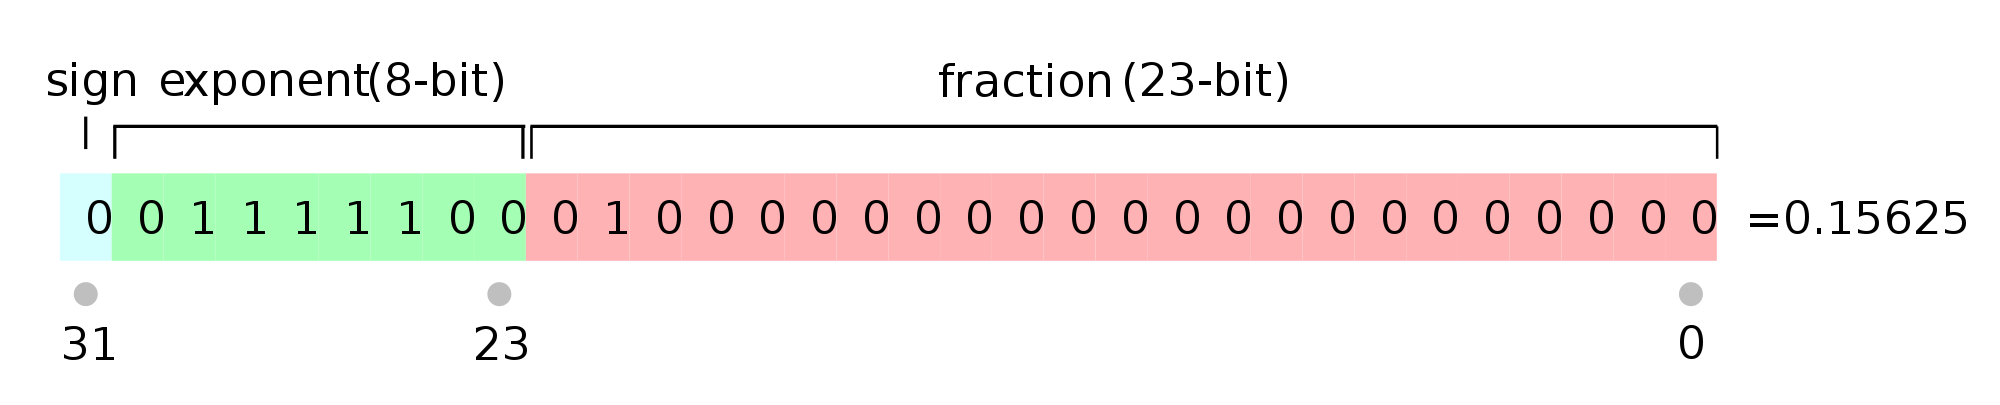
\includegraphics[width=\linewidth]{image/ieee-f32.png}
    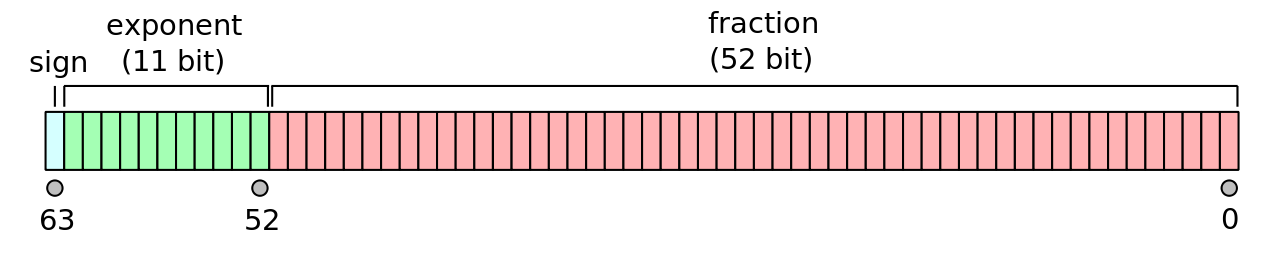
\includegraphics[width=\linewidth]{image/ieee-f64.png}
    \caption{IEEE 754 single (32 bits) and double (64 bits) precision floating
    point. \cite{ieee754-diagram}}
    \label{fig:ieee-f32}
\end{figure}

\subsection{Fused-multiply-add}
\label{sec:FMA}

After doing floating point arithmetic, it is required to normalize the result of
floating-point arithmetic before it can be used further. However, by feeding the
result of a floating-point multiplication (FMUL) directly into the
floating-point addition (FADD) logic without the need for normalization and
rounding in between, a fused multiply-add (FMA) operation is effectively
created: 
\begin{math}Y = (A * B) + C \end{math}, where 
\begin{math}A\end{math},
\begin{math}B\end{math} and
\begin{math}C\end{math} are the operands, 
 \begin{math}Y\end{math} is the result \cite{CARD}.

FMA saves cycles and reduces accumulation of rounding errors, while at the same
time not adding significant complexity to the circuit. A FMA execution unit is
capable to do FMUL, FADD, and FSUB as well: 
\begin{compactlist} 
\item[] Addition: \begin{math}Y = (A * 1.0) + C \end{math} 
\item[] Multiplication: \begin{math} Y = (A * B) + 0.0 \end{math} 
\item[] Subtraction: \begin{math} Y = (A * -1.0) + C\end{math} 
\end{compactlist} 

This is a useful feature in many numerical computations that involve
simultaneous multiplication and addition operations, such as dot product and
matrix multiplication. Since the pivot function performs multiplication and
addition between the pivot row, some constant value and each row in the matrix,
the performance of FMA is critical to the overall efficiency of the algorithm. 

\subsection{Representing ``\texttt{int23\_t}'' and ``\texttt{int52\_t}'' using
floating points}
\label{sec:fpe2}

There is a common stereotype that floating-point numbers are unreliable and
likely to be imprecise, and are often illustrated in popular memes (as shown in
Figure \ref{meme}). However, when storing integer values inside floating points, 
floating points can be quite reliable. 

Specifically, given that the mantissa part of a float consists of 23 bits,
inexactness never occur when representing integers less than 23 bits (ignoring
the sign bit). Furthermore, in case of of an integer overflow, floating point
imprecision almost always occurs and a corresponding status registers is set.
The same concept applies to double data types, which have a mantissa consisting
of 52 bits.

This mechanism is reliable, as floating-point inexactness always implies
integer-inexactness. For a integer value with bit width greater than the
mantissa size, floating point rounding is triggered in order to fit most
significant bits of the integer in the mantissa, and then adjust the order of
magnitude in the exponent accordingly. The lower bits of the mantissa are
truncated, therefore causing imprecision. 

In some rare cases, integers longer than the size of mantissa can be represented
in floating points precisely. An examples of such numbers are large powers of 2,
like \texttt{2\^{}30 = 0x40000000}. Its binary representation in \texttt{float}
is:
\begin{VerbatimCompact}
Sign    : 0
Exponent: 10011011
Mantissa: 00000000000000000000000
\end{VerbatimCompact}
Despite being greater than the size of
the mantissa, they are normalized rather then being rounded, and therefore does
not break the mechanism of representing integer in floating-points.

\begin{figure}
\begin{center}
    
\includegraphics[width=50mm,scale=0.1]{image/0.3004.jpg}
    \caption{A floating point meme: 0.1 + 0.2 = 0.30000000000000004}
    \label{meme}
\end{center}
\end{figure}


\subsection{Floating point exceptions and Fenv library}
\label{sec:fpe}
\hl{Arjun: I feel this is not really background, we are getting into the implementation now}

\section{Google Benchmark}
Google benchmark is a library to measure the performance of a code snippet. It
provides unit-test like interfaces to setup benchmarks around a code snippet
\cite{googlebench}. The given example from https://github.com/google/benchmark
is self-explanatory for its usage: 

\begin{verbatim}
#include <benchmark/benchmark.h>

static void BM_SomeFunction(benchmark::State& state) {
    // Perform setup here
    for (auto _ : state) {
    // This code gets timed
    SomeFunction();
    }
}
// Register the function as a benchmark
BENCHMARK(BM_SomeFunction);
// Run the benchmark
BENCHMARK_MAIN();
\end{verbatim}

The library first starts a timer, repeatedly executes its core loop: \texttt{for
(auto \_ : state) ... } multiple times then pauses the timer. This method
ensures that the results are consistent and minimizes the overhead required for
recording the timing information. 

Executing the benchmarks will not only report both elapsed real time and CPU
time, but also much other useful information to help reduce variance. 
\begin{verbatim}
Running ./build/example
***WARNING*** CPU scaling is enabled, the benchmark real time 
measurements may be noisy and will incur extra overhead.
Run on (32 X 5800.00 MHz CPU s)
CPU Caches:
    L1 Data 32 KiB (x16)
    L1 Instruction 32 KiB (x16)
    L2 Unified 1024 KiB (x16)
    L3 Unified 32768 KiB (x2)
Load Average: 8.10, 5.14, 1.14
----------------------------------------------------------
Benchmark                Time             CPU   Iterations
----------------------------------------------------------
BM_SomeFunction       18.5 ns         18.5 ns     37935734
\end{verbatim}

The warning: ``CPU scaling is enabled, the benchmark real-time measurements may
be noisy and will incur extra overhead.'' is saying that CPU clock frequency is
not consistent. It can be dynamically determined by the governor algorithm,
according on the system's needs. For example, with the \texttt{performance}
governor, the OS locks the CPU to the highest possible clock frequency,
specified at \texttt{/sys/devices/system/cpu/cpu*/cpufreq/scaling\_max\_freq},
while the \texttt{ondemand} governor will push the CPU to the highest frequency
on demand and then gradually reduce the frequency as the idle time increases
\cite{archLinuxFreqScal}.

However, it is also dependent on the manufacture and other hardware constraints.
By default, both Intel (Turbo Boost) and AMD (Precision Boost Overdrive) have
support for raising clock frequency, beyond the control of the governor
\cite{GoogleBenchReduceVariance}. On the other hand, CPUs have self-protecting
thermal throttling mechanisms that reduces its clock frequency and voltage when
it is too hot. 

The benchmark mentioned in this report were performed on a AMD 7950x desktop
computer. The computer system went through the following these setups for
consistent results:
\begin{compactlist}
    \item Set the governor to \texttt{performance}, 
    \item Disable AMD Precision Boost Overdrive (or Intel Turbo Boost), 
    \item Lock clock frequency at a 5 GHz, or any desired fixed value,
    \item Make sure heat dissipation is working properly.
\end{compactlist}



\section{\texttt{llvm-mca}}

\texttt{llvm-mca}, LLVM Machine Code Analyzer, is a tool to analyze performance of
executing some instructions on a specific CPU micro-architecture, according to
scheduling information provided by LLVM \cite{llvm-mca}. This tool may help with predicting and
explaining performance characteristics \hl{TODO: Is it necessary to mention mca?
Only use case is I found it not helpful}


\chapter{Experiments with Toy Example}
\label{sec:Toy}

The pivot function does multiply and add for each row in the matrix, therefore
the performance of FMA a simple vector toy can be an effective indicator. This
chapter reports performance analysis on simple toy examples that do vector add
or vector FMA with various setups, including: 

\begin{enumerate} 
    \item Vectorization method 
        \begin{compactlist} 
            \item Clang's automatic vectorization from scalar source code
            \item Clang builtin vector datatype with occasional AVX intrinsics 
        \end{compactlist}
    \item Matrix data structure 
        \begin{compactlist} 
            \item Nested list
            \item Flat list
        \end{compactlist}
    \item Element data width
        \begin{compactlist} 
            \item 16 bits: \texttt{int16\_t}
            \item 32 bits: \texttt{int32\_t}, \texttt{float}
            \item 64 bits: \texttt{int64\_t}, \texttt{double}
        \end{compactlist}
    \item Element data type 
        \begin{compactlist} 
            \item Integer
            \item Floating point
        \end{compactlist}
\end{enumerate}

\section{Vectorization method}

\subsection{Clang's automatic vectorization}
Clang is capable of generating vectorized instructions from scalar source code,
using the flags \texttt{-O3 -march=native} on a platform with vector ISA
enabled. Starting with an example (Listing \ref{vec-add-float-auto}), the simple
\texttt{vec\_add} function adds every element from two arrays and saves it to
the third. 

\begin{table}[ht]\captionsetup{name=Listing}
\begin{tabular}{>{\raggedright\arraybackslash}p{14cm}}
    Source code\\
    \midrule
    \begin{VerbatimCompact}
#define size 128
void vec_add(float* src1_ptr, float* src2_ptr, float* dst_ptr) {
    for (uint32_t i = 0; i < size; i += 1 ){
        dst_ptr[i] = src1_ptr[i] + src2_ptr[i];
    }
}
    \end{VerbatimCompact}
    \\

    Assembly snippet of the hot loop, compiled with \texttt{-O3 -march=native}
    (vectorization on)\\
    \midrule
    \begin{VerbatimCompact}
1458: c4 c1 7c 58 84 87 20   vaddps -0x1e0(%r15,%rax,4),%zmm0,%zmm0
145f: fe ff ff
1462: c4 c1 74 58 8c 87 40   vaddps -0x1a0(%r15,%rax,4),%zmm1,%zmm1
1469: fe ff ff
    \end{VerbatimCompact}
    \\

    Assembly snippet of the hot loop, compiled with \texttt{-O3 -march=native
    -mno-avx -mno-sse} (vectorization off)\\
    \midrule
    \begin{VerbatimCompact}
120d: d8 44 82 04    fadds  0x4(%rdx,%rax,4)
1211: d9 5c 81 04    fstps  0x4(%rcx,%rax,4)
1215: d9 44 86 08    flds   0x8(%rsi,%rax,4)
    \end{VerbatimCompact}
\end{tabular}
\caption{}
\label{vec-add-float-auto}
\end{table}
\hl{TODO: these hex code are actually incorrect, I assume this does not really matter?}

After compiling on a AVX-512 enabled computer and disassembling the binary, it
is observed that clang automatically packs 16 \texttt{float} (512 bits) as a
operand of the \texttt{VADDPS} instruction. 

Alternatively, vectorization could be disabled by adding the \texttt{-mno-avx
-mno-sse} flags on top of \texttt{-O3 -march=native}. These two sets of flags
guarantee that the binary are going to be equally optimized, with the only
difference been whether vector instructions are generated or not. In this case,
scalar instructions \texttt{fadds}, \texttt{fstps} and \texttt{flds} are
selected.


\subsection{Clang's vector datatype and AVX intrinsics}

Another approach is to write source code with vectorization in mind in the first
place. Clang provides extension that allows programmers to declare a new type
that represents a vector of elements of the same data type. The syntax is 
\begin{VerbatimCompact}[commandchars=\\\{\}]
typedef \textit{ty} \textit{vec_ty} __attribute__((ext_vector_type(\textit{vec_width}))), 
\end{VerbatimCompact}
where \textit{\texttt{vec\char`_ty}} is the name of vector type being defined,
\textit{\texttt{vec\char`_width}} is its size and \textit{\texttt{ty}} is the
type of the elements in the vector. For example, 
\begin{VerbatimCompact}[commandchars=\\\{\}]
typedef int16_t int16x32 __attribute__((ext_vector_type(32)))
\end{VerbatimCompact}
defines a 512-bit vector type of \texttt{int16x32}, consisting of 32
\texttt{int16\char`_t} and fits inside an AVX-512 ZMM register. 

After defining a vector datatype, a vector variable can be created by casting
from a pointer of the target array. Then arithmetic operators can be applied
between the vectors to performed element-wise operations. The previous
\texttt{vec\_add} example can be rewritten as the code snippet shown in Listing
\ref{vec-add-float-vecty}:

\begin{table}[ht]\captionsetup{name=Listing}
\begin{tabular}{>{\raggedright\arraybackslash}p{14cm}}
    Source code\\
    \midrule
    \begin{VerbatimCompact}
#define size 128
#define FloatZmmSize 16
typedef float floatZmm __attribute__((ext_vector_type(FloatZmmSize)));
void vec_add(float* src1_ptr, float* src2_ptr, float* dst_ptr) {
    for (uint32_t i = 0; i < size; i += FloatZmmSize ){
        floatZmm src1Vec = *(floatZmm *)(src1_ptr + i);
        floatZmm src2Vec = *(floatZmm*)(src2_ptr + i);
        floatZmm resultVec = src1Vec + src2Vec;
        *(floatZmm *)(dst_ptr + i) = resultVec;
    }
}
\end{VerbatimCompact}
\end{tabular}
\caption{}
\label{vec-add-float-vecty}
\end{table}
\subsection{Evaluation}
When comparing the performance of code written with and without the vector type
and examining their assembly, it has been discovered that the the automatic
vectorization feature in clang can be unpredictable and may lead to undesired
behaviors. It operates as a black box and may take a lot of effort to understand
its mechanisms. One of the issues is that clang may select a suboptimal vector
width.

Consider the \texttt{vec\_fma} function in Listing
\ref{table:vec-fma-float-auto} and \ref{table:vec-fma-float-vecty}, a slightly
more complicated version of the previous \texttt{vec\_add} example, where an
additional array is introduced and the element-wise operation is changed from
addition to FMA. The disassembly reveals that clang decides to use FMA vector
instructions of 128-bit width, but when vector size is constrained to 512-bit
width by defining a vector type, more optimal binary can be generated. Benchmark
indicates that the 512-bit vector width version is xx\% faster.  
\hl{TODO: determine this number}


% 80e4: c5 fa 10 04 b2       	vmovss (%rdx,%rsi,4),%xmm0
% 80e9: 43 8d b4 2f 8b 00 00 	lea    0x8b(%r15,%r13,1),%esi
% 80f0: 00 
% 80f1: c5 fa 10 0c 81       	vmovss (%rcx,%rax,4),%xmm1
% 80f6: 43 8d 84 2b 8a 00 00 	lea    0x8a(%r11,%r13,1),%eax
% 80fd: 00 
% 80fe: c4 c2 79 a9 0c b8    	vfmadd213ss (%r8,%rdi,4),%xmm0,%xmm1
% 8104: 42 8d bc 2b 8b 00 00 	lea    0x8b(%rbx,%r13,1),%edi
% 810b: 00 
% 810c: c4 c1 7a 11 0c 81    	vmovss %xmm1,(%r9,%rax,4)
% 8112: 43 8d 84 2e 8b 00 00 	lea    0x8b(%r14,%r13,1),%eax
% 8119: 00 

\begin{table}[ht]\captionsetup{name=Listing}
\begin{tabular}{>{\raggedright\arraybackslash}p{14cm}}
    Source code\\
    \midrule
    \begin{VerbatimCompact}
void vec_fma(float* src1_ptr, float* src2_ptr,
             float* src3_ptr, float* dst_ptr) {
    for (uint32_t i = 0; i < size; i += 1 ){
        dst_ptr[i] = src1_ptr[i] * src2_ptr[i] + src3_ptr[i];
    }
}
    \end{VerbatimCompact}
    \\
    % \toprule
    Assembly snippet of the hot loop\\
    \midrule
    \begin{VerbatimCompact}
80e4: c5 fa 10 04 b2     vmovss (%rdx,%rsi,4),%xmm0
80f1: c5 fa 10 0c 81     vmovss (%rcx,%rax,4),%xmm1
80fe: c4 c2 79 a9 0c b8  vfmadd213ss (%r8,%rdi,4),%xmm0,%xmm1
810c: c4 c1 7a 11 0c 81  vmovss %xmm1,(%r9,%rax,4)
    \end{VerbatimCompact}
    \\
\end{tabular}
\caption{}
\label{table:vec-fma-float-auto}
\end{table}

\begin{table}[H]\captionsetup{name=Listing}
\begin{tabular}{>{\raggedright\arraybackslash}p{14cm}}
    Source code\\
    \midrule
    \begin{VerbatimCompact}
#define size 128
#define FloatZmmSize 16
typedef float floatZmm __attribute__((ext_vector_type(FloatZmmSize)));
void vec_fma(float* src1_ptr, float* src2_ptr,
             float* src3_ptr, float* dst_ptr) {
    for (uint32_t i = 0; i < size; i += 1 ){
        floatZmm src1Vec = *(floatZmm *)(src1_ptr + i);
        floatZmm src2Vec = *(floatZmm *)(src2_ptr + i);
        floatZmm src3Vec = *(floatZmm *)(src3_ptr + i);
        *(floatZmm *)(dst_ptr + i) = src1Vec * src2Vec + src3Vec;
    }
}
    \end{VerbatimCompact}
    \\
    % \toprule
    Assembly snippet of the hot loop\\
    \midrule
    \begin{VerbatimCompact}
82c0: 62 b1 7c 48 10 04 80   vmovups (%rax,%r8,4),%zmm0
82c7: 62 b1 7c 48 10 0c 81   vmovups (%rcx,%r8,4),%zmm1
82ce: 62 b2 7d 48 a8 0c 86   vfmadd213ps (%rsi,%r8,4),%zmm0,%zmm1
82d5: 62 b1 7c 48 11 0c 87   vmovups %zmm1,(%rdi,%r8,4)
    \end{VerbatimCompact}
    \\
\end{tabular}
\caption{}
\label{table:vec-fma-float-vecty}
\end{table}
    



In some cases clang could be even worse, it may fail to recognize vectorization
patterns from element-wise loop operations, leading to more reduction in
performance. In the \texttt{vec\_fma} example, by changing the type signature
from \texttt{float} to \texttt{int}, clang decides to dispatch scalar
instructions for addition (\texttt{add}) and multiplication (\texttt{imul})
completely (Listing \ref{vec-fma-int-auto}). Their vectorized equivalency
\texttt{vpaddd} and \texttt{vpmulld} are more performant options. (Listing
\ref{vec-fma-int-auto}).

\begin{table}[ht]\captionsetup{name=Listing}
\begin{tabular}{>{\raggedright\arraybackslash}p{14cm}}
    Source code\\
    \midrule
    \begin{VerbatimCompact}
#define size 128
void vec_fma(int* src1_ptr, int* src2_ptr, 
             int* src3_ptr, int* dst_ptr) {
    for (uint32_t i = 0; i < size; i += 1 ){
        dst_ptr[i] = src1_ptr[i] * src2_ptr[i] + src3_ptr[i];
    }
}
    \end{VerbatimCompact}
    \\
    % \toprule
    Assembly snippet of the hot loop\\
    \midrule
    \begin{VerbatimCompact}
88b0: 44 8b 69 1c  mov    0x1c(%rcx),%r13d
88b4: 44 8b 62 1c  mov    0x1c(%rdx),%r12d
88b8: 45 0f af ee  imul   %r14d,%r13d
88bc: 45 0f af e6  imul   %r14d,%r12d
88c0: 45 01 fd     add    %r15d,%r13d
88c3: 45 01 fc     add    %r15d,%r12d
    \end{VerbatimCompact}
    \\
\end{tabular}
\caption{}
\label{vec-fma-int-auto}
\end{table}

\begin{table}[H]\captionsetup{name=Listing}
\begin{tabular}{>{\raggedright\arraybackslash}p{14cm}}
    Source code\\
    \midrule
    \begin{VerbatimCompact}
#define size 128
#define IntZmmSize 16
typedef int intZmm __attribute__((ext_vector_type(IntZmmSize)));
void vec_fma(int* src1_ptr, int* src2_ptr,
             int* src3_ptr, int* dst_ptr) {
    for (uint32_t i = 0; i < size; i += 1 ){
        intZmm src1Vec = *(intZmm *)(src1_ptr + i);
        intZmm src2Vec = *(intZmm *)(src2_ptr + i);
        intZmm src3Vec = *(intZmm *)(src3_ptr + i);
        *(intZmm *)(dst_ptr + i) = src1Vec * src2Vec + src3Vec;
    }
}
    \end{VerbatimCompact}
    \\
    % \toprule
    Assembly snippet of the hot loop\\
    \midrule
    \begin{VerbatimCompact}
8880: 62 b1 fe 48 6f 04 81  vmovdqu64 (%rcx,%r8,4),%zmm0
8887: 62 b2 7d 48 40 04 80  vpmulld (%rax,%r8,4),%zmm0,%zmm0
888e: 62 b1 7d 48 fe 04 86  vpaddd (%rsi,%r8,4),%zmm0,%zmm0
8895: 62 b1 fe 48 7f 04 87  vmovdqu64 %zmm0,(%rdi,%r8,4)
    \end{VerbatimCompact}
    \\
\end{tabular}
\caption{}
\label{vec-fma-int-vecty}
\end{table}


% \begin{verbatim}
% #define size 128
% #define IntZmmSize 16
% typedef int intZmm __attribute__((ext_vector_type(IntZmmSize)));
% void vec_fma(int* src1_ptr, int* src2_ptr, 
%              int* src3_ptr, int* dst_ptr) {
%     for (uint32_t i = 0; i < size; i += 1 ){
%         intZmm src1Vec = *(Zmm *)(src1_ptr + i);
%         intZmm src2Vec = *(Zmm *)(src2_ptr + i);
%         intZmm src3Vec = *(Zmm *)(src3_ptr + i);
%         *(intZmm *)(dst_ptr + i) = src1Vec * src2Vec + src3Vec;
%     }
% }
% \end{verbatim}


\section{Matrix data structure}

The most intuitive data structure of a matrix is a list of lists, where each
list represents a row and a list of rows is a matrix. In C++ this can be
represented using \texttt{std::vector<std::vector<T>>}, where \texttt{T} could
be \texttt{float}, \texttt{double}, \texttt{int32\_t}, etc. The std::vector
class provides an intuitive interface for accessing and modifying elements,
making it easy to write code with. 

One potential drawback of nested \texttt{std::vector} is that it requires two
indexing operations to access an element. An alternative implementation is to
“flatten” a matrix into a single \texttt{std::vector}, by simply concatenating
one row after another. To access a specific element, an index can be computed
manually using the given row and column: \texttt{column\_count * row + column}.
This reduces half of the memory indexing operation at the cost of additional
arithmetic. The differences between the two patterns are illustrated by a
example provided in Table \ref{table:nested-flat}. 

\begin{table}[ht]

\begin{tabular}{%
    >{\raggedright\arraybackslash}p{2cm}%
    >{\raggedright\arraybackslash}p{6.5cm}%
    >{\raggedright\arraybackslash}p{4.5cm}}
    
    \toprule
    & Nested & Flat\\

    \midrule
    
    Type
    &
    \begin{VerbatimCompact}
std::vector<
    std::vector<int32_t>>
    \end{VerbatimCompact}
    &
    \begin{VerbatimCompact}
std::vector<int32_t>
    \end{VerbatimCompact}
    \\

Structure in Memory
    &
    \begin{VerbatimCompact}
vector of 4 = {
    vector of 4 = {0, 0, 0, 0}, 
    vector of 4 = {0, 0, 0, 0}, 
    vector of 4 = {0, 0, 0, 1}, 
    vector of 4 = {0, 0, 0, 0}
}
    \end{VerbatimCompact}
    &
    \begin{VerbatimCompact}
vector of 16 = {
    0, 0, 0, 0, 
    0, 0, 0, 0,
    0, 0, 0, 1, 
    0, 0, 0, 0
}
    \end{VerbatimCompact}
    \\

    Accessing row 2, column 3
    &
    Index row first: \texttt{std::vector<int32\_t>[2]} \linebreak
    then index column: 
        \texttt{std::vector<int32\_t>[2][3]}
    & 
    Compute \texttt{i = 
    \linebreak col\_count * row + col \linebreak = 4 * 2 + 3 =
    11}, \linebreak then index once: \texttt{std::vector<int32\_t>[11]}  \\

    \bottomrule

\end{tabular}
\caption{This is an example of a 4 by 4 matrix, to highlight the differences
between the two matrix data structures: nested list and flat list. }
\label{table:nested-flat}
\end{table}

Empirically indexing costs more time than integer multiplication and addition,
thereby improving performance. Both the toy example and the pivot function
perform sequential load-compute-store operations on each row and each column,
allowing the index of the next element to be computed by simply adding the step
size or column size, further reducing memory overhead. In fact, the pivot
function can be optimized to only compute index once (See Section
\ref{sec:optmz-get-index}) by placing the pivot row as first row. Benchmark
(Figure \ref{fig:nested-flat}) on the toy example confirms that when there are
16 rows, the nested vector matrix is about 8 ns faster than the flat matrix.

\begin{figure}
    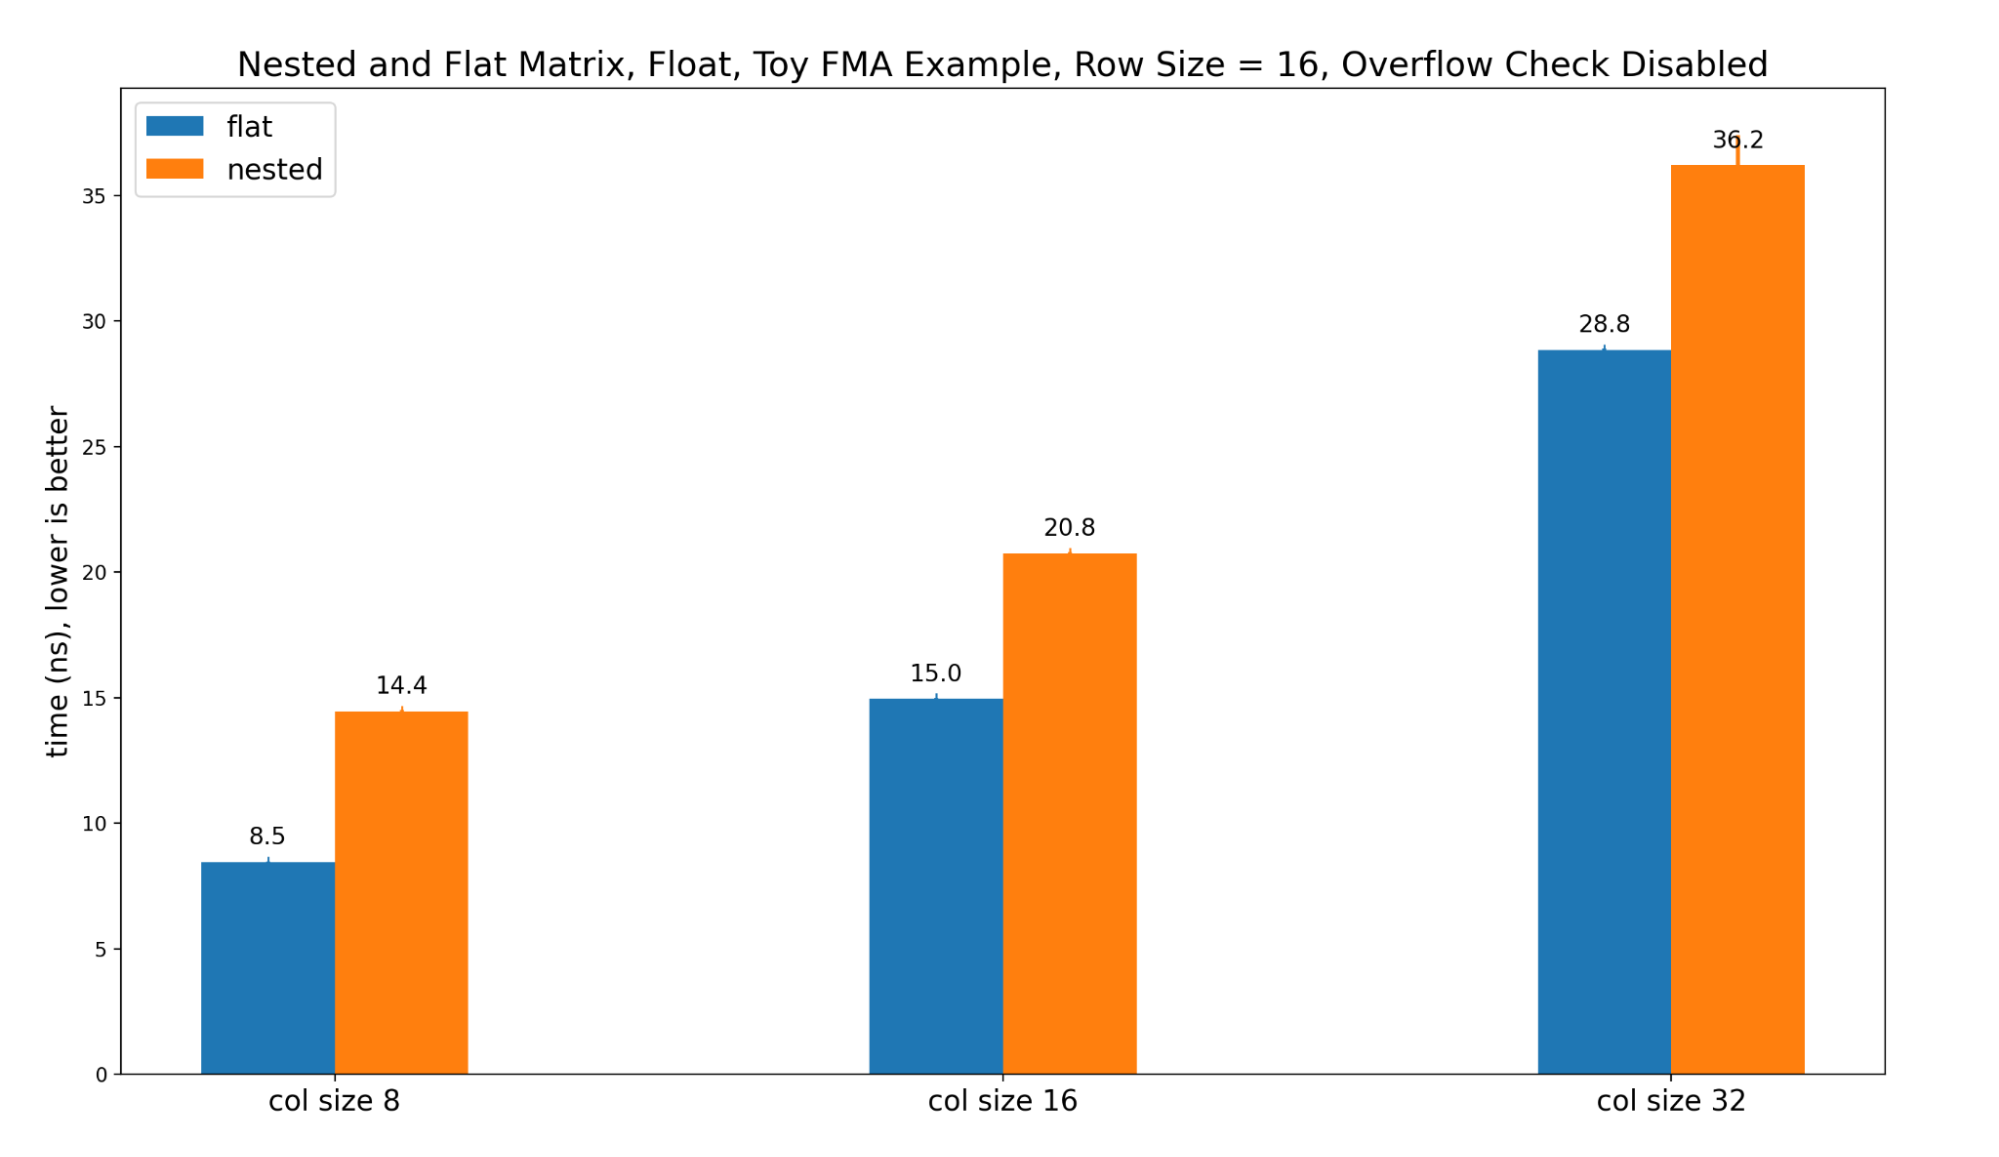
\includegraphics[width=\linewidth]{image/nested-flat.jpg}
    \caption{\hl{TODO: write caption}}
    \label{fig:nested-flat}
\end{figure}


\section{Matrix element data type}


\subsection{Width}
Since the numbers stored in the matrix are almost always less than 10 bits,
using shorter data types can be more advantageous than longer ones because they
allow more numbers to be packed into a single vector register (Table
\ref{archtable}). The number of instructions can be cut by half when data width
is reduced to half, and less instruction count always leads to less execution
time. Given that the Zen4 micro-architecture provides approximately same amount
of execution units for both integers and floating points, it is reasonable to
estimate that the execution time is inversely proportional to the bit width of
data type. As confirmed in Plot \ref{fig:col8-col16-col32-i16-i32-f32-f64},
\texttt{int32\_t} and \texttt{float} costs nearly same amount of time, while
\texttt{int32\_t} and \texttt{double} costs double the amount of time than
\texttt{int16\_t} and \texttt{float} respectively.


\begin{figure}[H]
    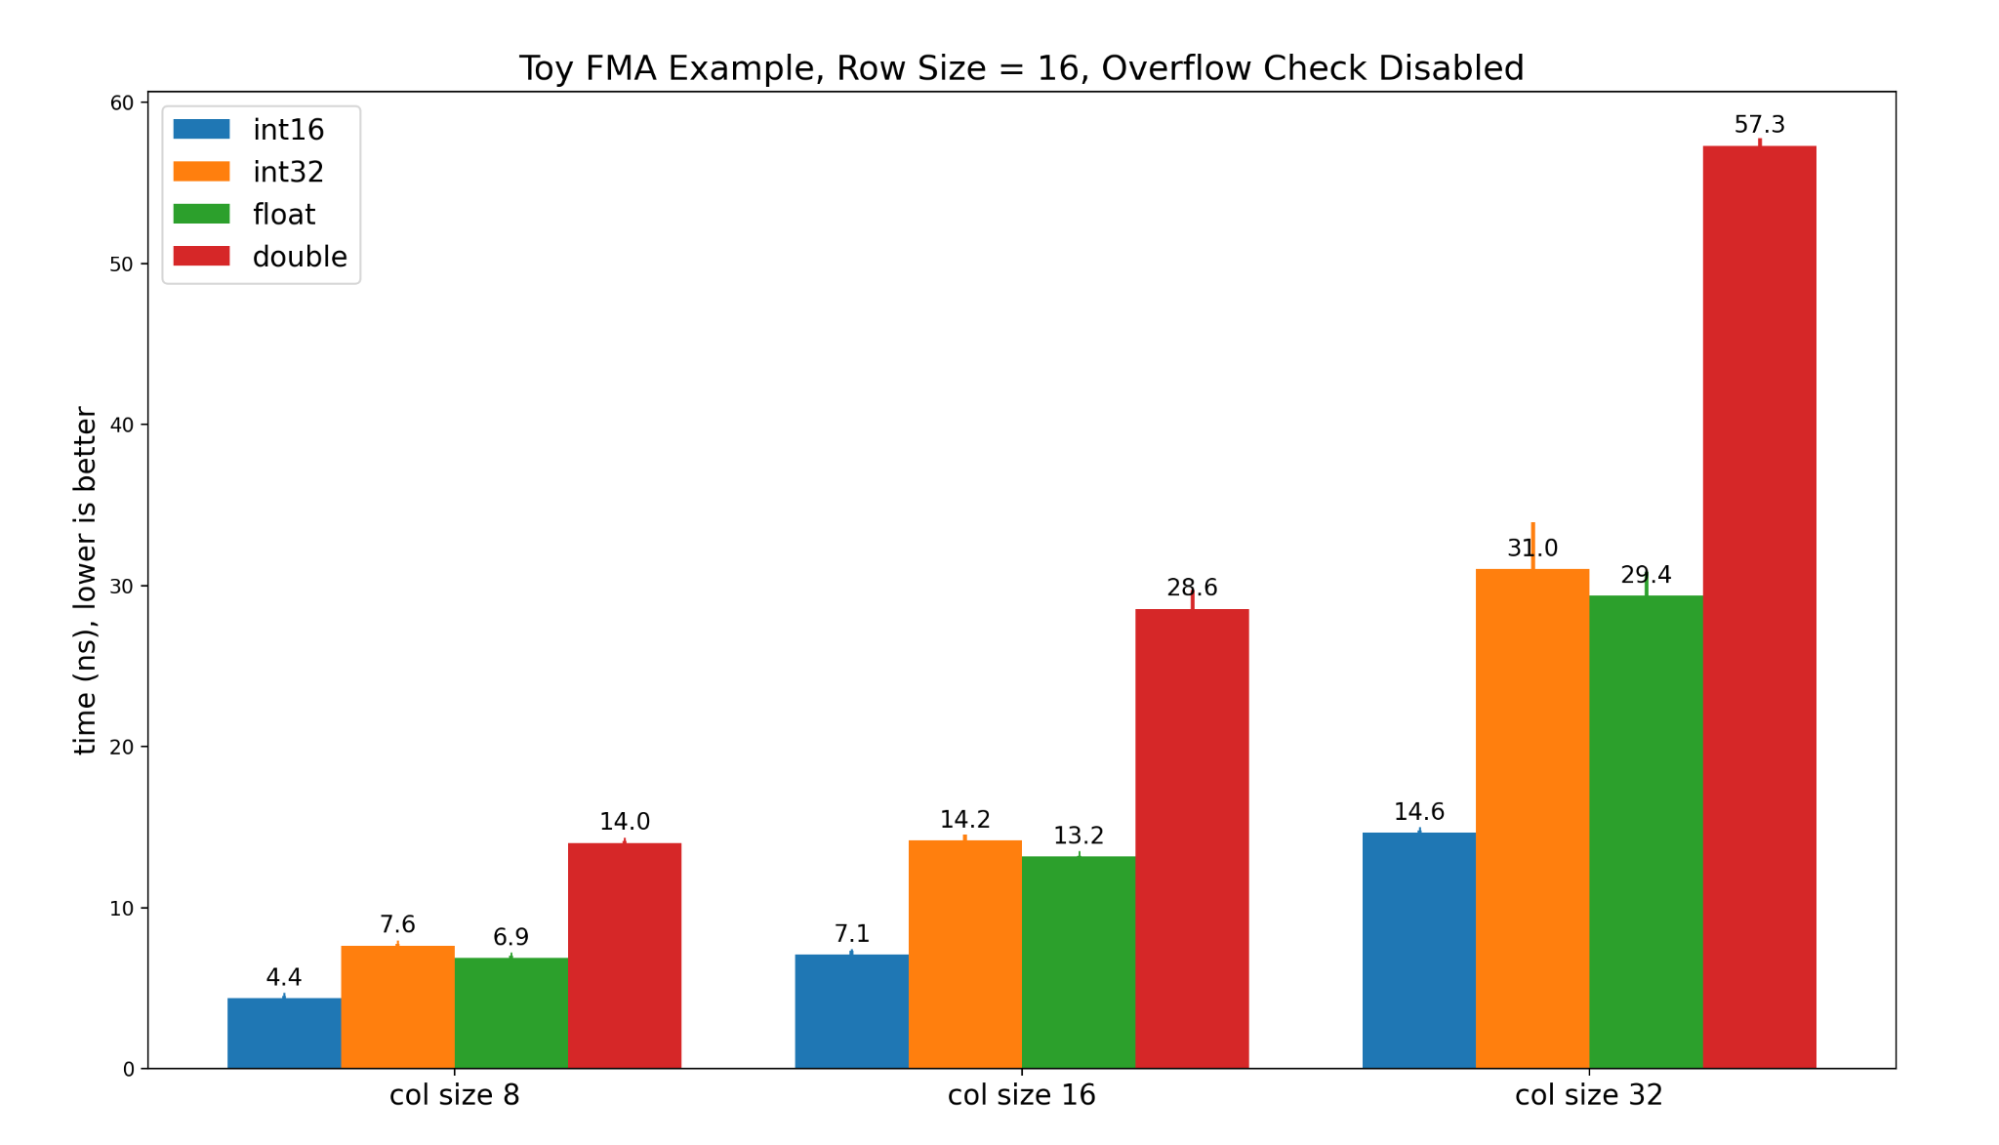
\includegraphics[width=\linewidth]{image/col8-col16-col32-i16-i32-f32-f64.png}
    \caption{\hl{TODO: write caption}}
    \label{fig:col8-col16-col32-i16-i32-f32-f64}
\end{figure}

\begin{figure}[H]\captionsetup{name=}
    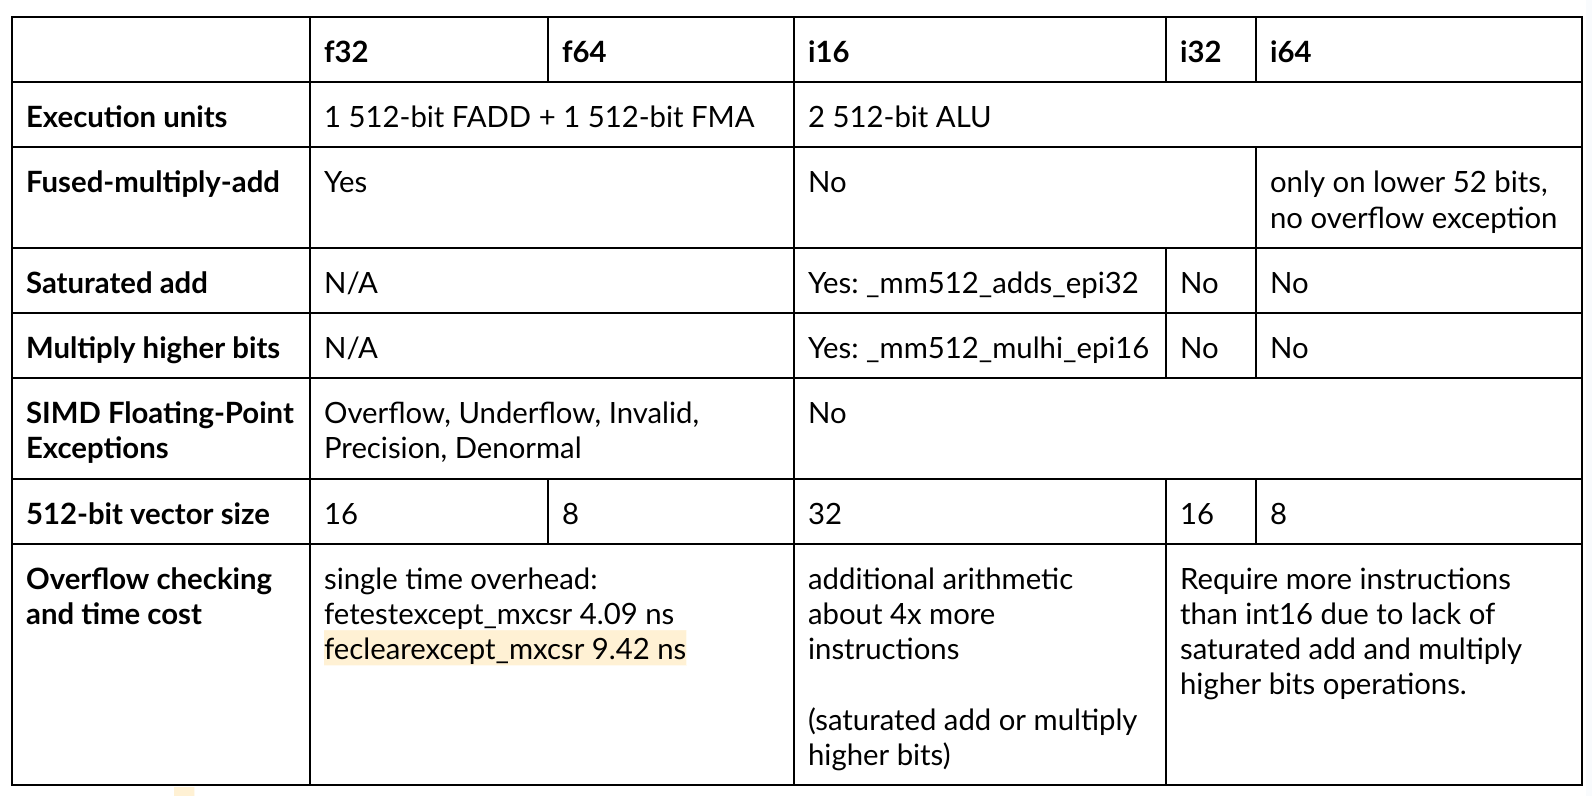
\includegraphics[width=\linewidth]{image/arch-table.png}
    \caption{\hl{TODO: write caption}}
    \label{archtable}
\end{figure}

\subsection{Overflow checking for integers}

The x86-64 micro-architecture provides the \texttt{seto} instruction to set some
byte to \texttt{1} if overflow occurred as a result of integer arithmetic.
However \texttt{seto} only works for scalar operations, there does not exist
instruction or status register to indicate whether a previous vector add or
multiply instruction produces overflown results or not. Therefore, overflow has
to be checked manually by some additional vector instructions, this would slow
down the computation to some extent. Or alternatively or arithmetics have to be
carried out on each element individually in a scalar manner,resulting in even
worse performance. 


% One advantage of using \texttt{int16\_t} is that it can be used with AVX-512's
% saturated add and multiply higher bits vector instructions, which are listed in
% Table \ref{archtable}. This allows for the creation of vectorized code that
% takes overflow into account and is therefore more efficient. However, it should
% be noted that there are no equivalent instructions for \texttt{int32_t} and
% \texttt{int64_t}.

One advantage of \texttt{int16\_t} is that it can be used with AVX-512's
saturated add and multiply higher bits vector instructions (Table
\ref{archtable}), making it possible and convenient to write vectorized and
overflow-aware code. However, Zen4's implementation of AVX-512 extension does
not provide equivalent instruction for \texttt{int32\_t} or \texttt{int64\_t},
and therefore must be processed as scalar values.
% When the
% result of a conventional add does not match the result of a saturated add, or
% when multiplying for the higher 16 bits gives non-zero results, it implies an
% overflow. 


% \subsection{Implementation of detecting overflow for \texttt{int16\_t} }
\subsubsection{Implementation of vectorized \texttt{int16\_t} overflow checking}
By comparing the result of a conventional addition and saturated addition, it
indicates whether an addition has gone overflown or not. In case of overflow,
with saturated add, the result always retains at the maximum possible value of
\texttt{int16\_t}: \texttt{0x7FFF}, while the result of a conventional add is
always smaller, because the overflowed output from conventional addition can't
go all the way around and become \texttt{INT16\_MAX} again. In the two's
complement binary form for integer, the overflow sum is "trapped" in the
negative number space. For example: 
\begin{verbatim}
INT16_MAX + 1 = INT16_MIN = -32768, 
INT16_MAX + 2 = -32767, 
...
INT16_MAX + INT16_MAX = -2, 
\end{verbatim}

For multiplication, as two 16-bit numbers produces 32-bit products but only
lower 16 bits can be stored, overflow can be detected by checking whether any of
the upper 16 bits are set. 

Inspecting these approaches from a instruction-level perspective (Table
\ref{table:i16-instr}), when overflow is ignored, both add and multiply takes 1
instruction, 
\hlc[pink]{\texttt{vpaddw}}\footnote{Vector add for \texttt{int16\_t}} 
and 
\hlc[pink]{\texttt{vpmullw}}\footnote{Vector multiply lower half bits for \texttt{int16\_t}}. 
To obtain and process overflow-related
information, an additional computation instruction
\hl{\texttt{vpaddsw}}\footnote{Vector saturated add for \texttt{int16\_t}}
or
\hl{\texttt{vpmulhw}}\footnote{Vector multiple higher half bits for \texttt{int16\_t}} 
is required, followed with 2 or 3 comparison, shuffling and branch instructions:
\hlc[cyan!60]{\texttt{vpsraw}}\footnote{Shift packed data right arithmetic},
\hlc[cyan!60]{\texttt{vpcmpneqw}}\footnote{Compare packed data for equal}
and 
By enabling
\hlc[cyan!60]{\texttt{kord}}\footnote{Bitwise logical OR masks}. 
overflow checking, it brings  4x or 5x more instruction count and 60\% more
runtime \cite{FPL2}. \hl{(TODO: verify this number?)}

\begin{center}
\begin{table}[ht]

\begin{tabular}{  c  L{5.5cm} L{5.5cm}  } 
     & Addition & Multiplication \\ 
    \midrule
        Disabled 
    & 
        \hlc[pink]{\texttt{vpaddw \%zmm4,\%zmm2,\%zmm3}} 
    &
        \hlc[pink]{\texttt{vpmullw \%zmm1,\%zmm3,\%zmm2}} \\
    \midrule
        Enabled 
    &
        \hlc[pink]{\texttt{vpaddw \%zmm4,\%zmm2,\%zmm3}}
        \hl{\texttt{vpaddsw \%zmm2,\%zmm4,\%zmm2}}
        \hlc[cyan!60]{\texttt{vpcmpneqw \%zmm3,\%zmm2,\%k1}}
        \hlc[cyan!60]{\texttt{kord \%k1,\%k0,\%k0}}
    &  
        \hlc[pink]{\texttt{vpmullw \%zmm1,\%zmm3,\%zmm2}}
        \hl{\texttt{vpmulhw \%zmm1,\%zmm3,\%zmm3}}
        \hlc[cyan!60]{\texttt{vpsraw \$0xf,\%zmm2,\%zmm5}}
        \hlc[cyan!60]{\texttt{vpcmpneqw \%zmm3,\%zmm5,\%k1}}
        \hlc[cyan!60]{\texttt{kord \%k0,\%k1,\%k0}} \\
  \end{tabular}
  \caption{\hl{(TODO: write caption)}}
  \label{table:i16-instr}
\end{table}
\end{center}

\subsubsection{Implementation of scalar \texttt{int32\_t} and \texttt{int64\_t}
overflow checking} 

Clang's language extension provides functions to perform overflow-checked
integer arithmetics: 
\begin{VerbatimCompact}
bool __builtin_add_overflow (type1 x, type2 y, type3 *sum);
bool __builtin_mul_overflow (type1 x, type2 y, type3 *prod);
\end{VerbatimCompact}
These functions take three arguments: \texttt{x} and \texttt{y} are the two
input operands, and \texttt{sum} or \texttt{prod} is a pointer to the variable
that will hold the result of the addition or multiplication. The return value of
these functions is a boolean that indicates whether an overflow occurred during
the operation.

\subsubsection{Performance comparison}
\hl{TODO: write benchmark and plot! I have not done such benchmark ever}

\subsection{Overflow checking for floating points}
Integers and floating points have distinct mechanisms for overflow checking

\chapter{Pivot}

\section{Optimization}
\subsection{Alignment}
\subsection{Vector size specialization}
\subsection{Reduce floating point status register manipulation}
\subsection{Reduce number of matrix index computation}
\label{sec:optmz-get-index}


\chapter{Conclusions}

\section{Final Reminder}

The body of your dissertation, before the references and any appendices,
\emph{must} finish by page~40. The introduction, after preliminary material,
should have started on page~1.

You may not change the dissertation format (e.g., reduce the font size, change
the margins, or reduce the line spacing from the default single spacing). Be
careful if you copy-paste packages into your document preamble from elsewhere.
Some \LaTeX{} packages, such as \texttt{fullpage} or \texttt{savetrees}, change
the margins of your document. Do not include them!

Over-length or incorrectly-formatted dissertations will not be accepted and you
would have to modify your dissertation and resubmit. You cannot assume we will
check your submission before the final deadline and if it requires resubmission
after the deadline to conform to the page and style requirements you will be
subject to the usual late penalties based on your final submission time.

\bibliographystyle{plain}
\bibliography{mybibfile}


% You may delete everything from \appendix up to \end{document} if you don't need it.
% \appendix

% \chapter{First appendix}

% \section{First section}

% Any appendices, including any required ethics information, should be included
% after the references.

% Markers do not have to consider appendices. Make sure that your contributions
% are made clear in the main body of the dissertation (within the page limit).

% \chapter{Participants' information sheet}

% If you had human participants, include key information that they were given in
% an appendix, and point to it from the ethics declaration.

% \chapter{Participants' consent form}

% If you had human participants, include information about how consent was
% gathered in an appendix, and point to it from the ethics declaration.
% This information is often a copy of a consent form.


\end{document}
